\subsection{Graphical user interface}

The graphical user interface application is written in python since it often means faster development iterations. To fit the cross-platform requirements, the ui framework Qt[ref] is used. The core of Qt is written in C++ but there are python bindings available. Gpuip uses pyside[ref] since they are well documented and supported on the offical Qt homepage. 
\newline

\begin{figure}[ht!]
\centering
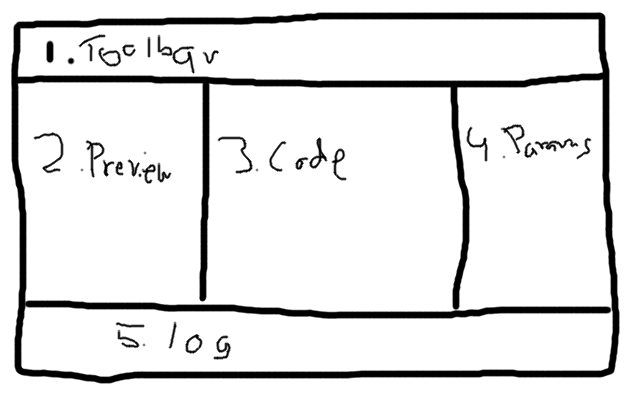
\includegraphics[width=90mm]{img/gui.png}
\caption{GUI sketch}
\label{guisketch}
\end{figure}

Figure \ref{guisketch} shows a sketch of the inital GUI ideas. The application will be a {\tt QMainWindow}. Main windows in Qt support menus and toolbars. All the different components will be dock widgets. A dock widget is resizeable and can be deattached to a solo window. The following compontents will be added as dock widgets.

\begin{enumerate}
\item Toolbar. Add menu items and toolbar items as {\tt QAction}. It is possible to bind an action to a hotkey.
\item Preview. Display the content of a buffer using {\tt QGLWidget}. Supports zoom and pan. If the image has floating point precision, a slider controlling the exposure is added. This is based on the same display algorithm as exrdisplay[ref].
\item Code. This is a {\tt QTextEdit} containing the kernel code. When building a kernel, gpuip reads the text from this widget.
\item Params. Per kernel setup with {\tt QComboBox} dropdown menus for buffer selection and parameter value with {\tt QSlider} and {\tt QLineEdit}.
\item Log. Output log for all commands using {\tt QTextBrowser}.
\end{enumerate}
